\documentclass{beamer}
\usepackage{times, amsthm, amsmath, amssymb, cancel, changepage, graphicx, lipsum, fancyhdr, mathabx, enumitem,caption, subcaption}
\usetheme{CambridgeUS}
\usecolortheme{seagull}
\usefonttheme{serif}
\definecolor{navy}{RGB}{0, 0, 128} 
\setbeamercolor{frametitle}{fg=navy}
\setbeamercolor{title}{fg=navy}
\setbeamerfont{frametitle}{series=\bfseries}
\setbeamerfont{title}{series=\bfseries}


\title{Lecture 6: Sequences \& Series II}
\date{September 12, 2019}

\begin{document}
	
\frame{\titlepage}

\begin{frame}
\frametitle{Series With Positive Terms}
\begin{itemize}
	\item[(i)] If $a_i \geq 0$ for all $i$, then the partial sums $S_n$ must be non-decreasing
	\item[(ii)] If the $S_n$'s are to approach a limit they cannot become arbitrarily large.
\end{itemize}
Suppose there exists some $B \geq S_n$ for all $n$, then $B$ is called an upper bound of the sequence $\{S_n\}$. The sequence is bounded. If $B' < B$ such that $S_n > B'$. $B$ is then called the least upper bound and 
$$\sum_{n=1}^\infty a_n = B$$
Can characterize the sum of a infinte series as
$$\lim\limits_{n \to \infty} \sum_{i=1}^n a_i \mbox{ or } \sup_{n=1}^\infty \{S_n\}$$

\end{frame}

\begin{frame}
\frametitle{Tests of Convergence: Integral Test}
If $f$ is a continuous, positive, decreasing function on $[k,\infty]$ and $a_n = f(n)$, then the series $\sum_{n=k}^\infty a_n$ is convergent if and only if the improper integral $\int_k^\infty f(x)\mathop{dx}$ is convergent.

\vspace{12pt}
\textbf{Examples:}
\begin{itemize}
	\item[(a)] $\sum_{n=1}^\infty n e^{-n^2}$
	\item[(b)] $\sum_{n=0}^\infty \frac{n^2}{n^3+1}$
	\item[(c)] For what values of $p$ does the series $\sum_{n=1}^\infty \frac{1}{x^p}$ converge?
\end{itemize}
\end{frame}

\begin{frame}
\frametitle{Tests of Convergence: Limit Comparison Test}
Suppose $\sum a_n$ and $\sum  b_n$ are series with positive terms. Then
\begin{itemize}
	\item[(i)] If $\lim\limits_{n \to \infty} \frac{a_n}{b_n} = c> 0$, then either both series converge or diverge.
	\item[(ii)] If $\lim\limits_{n \to \infty} \frac{a_n}{b_n} =  0$ and $\sum  b_n$ converges, then $\sum  a_n$ converges.
	\item[(iii)] If $\lim\limits_{n \to \infty} \frac{a_n}{b_n} =  \infty$ and $\sum  b_n$ diverges then $\sum a_n$ diverges.
\end{itemize}

\vspace{12pt}
\textbf{Examples:}
\begin{itemize}
	\item[(a)] Test $\sum_{n=1}^\infty \frac{1}{2^n-1}$ for convergence.
	\item[(b)] Test $\sum_{n=1}^\infty \frac{\ln n}{n}$ for convergence.
	\item[(c)] Test $\sum_{n=3}^\infty \frac{e^{-n}}{n^2 + 2n}$ for convergence.
\end{itemize}
\end{frame}

\begin{frame}
\frametitle{Tests of Convergence: Ratio Test}
Let $a_n$ be any sequence
\begin{itemize}
	\item[(i)] If $\lim_{n\to \infty} |\frac{a_{n+1}}{a_n}| = L < 1$ then the series $\sum a_n$ is convergent.
	\item[(ii)] If $\lim_{n\to \infty} |\frac{a_{n+1}}{a_n}| = L > 1$ then the series $\sum a_n$ is divergent.
	\item[(iii)] If $\lim_{n\to \infty} |\frac{a_{n+1}}{a_n}| =  1$ then the test fails.
\end{itemize}

\vspace{12pt}
\textbf{Examples:}
\begin{itemize}
	\item[(a)] Test $\sum_{n=1}^\infty \frac{n^n}{n!}$ for convergence
	\item[(b)] Test $\sum_{n=3}^\infty \frac{e^{4n}}{(n-2)!}$ for convergence
	\item[(c)] Test $\sum_{n=1}^\infty \frac{(-1)^{n+1}}{6n+7}$ for convergence
\end{itemize}
\end{frame}

\begin{frame}
\frametitle{Absolute Convergence}
Consider any sequence $a_1, a_2,...$. A series $\sum_{n=1}^\infty a_n$ convergences absolutely if the series $\sum_{n=1}^\infty |a_n|$ converges.

\vspace{12pt}
\textbf{Examples:}
\begin{itemize}
	\item[(a)] Test $\sum_{n=1}^\infty \frac{(-1)^{n+2}}{n^2}$ for absolute convergence
	\item[(b)]  Test $\sum_{n=1}^\infty \frac{(-1)^n}{n}$ for absolute convergence
\end{itemize}
\end{frame}


\begin{frame}
\frametitle{Strategies for Testing Series}
Classify according to the form of the series
\begin{itemize}
	\item[(1)] P-series $\sum \frac{1}{n^p}$ is convergent if $p>1$ and divergent if $p \leq 1$
	\item[(2)] Geometric series $\sum ar^{n-1}$ or $\sum ar^n$ is convergent if $|r| < 1$ and divergent if $|r| \geq 1$
	\item[(3)] If the series has the form that is similar to (1) or (2), then use the limit comparison test
	\item[(4)] If you can notice that $\lim\limits_{n \to \infty} a_n \neq 0$ then use the test for divergence theorem
	\item[(5)] For series involving factorials or other products, use the ratio test
	\item[(6)] If $a_n = f(n)$ and $\int_k^\infty f(x) \mathop{dx}$ is easy to evaluate, use the integral test
\end{itemize}
\end{frame}

\begin{frame}
\frametitle{Power Series}
Let $x$ be any number and $\{a_n\}$ by a sequence of numbers. A power series is any series of the form 
$$\sum_{n=1}^\infty a_n x^n$$
with partial sums $S_n = a_0 + a_1x + a_2x^2 + ... + a_nx^n$

\vspace{12pt}
\textbf{Examples:}
\begin{itemize}
	\item[(a)] For what values of $x$ does the series $\sum_{n=0}^\infty rx^n$ converge?
	\item[(b)] For what values of $x$ does the series $\sum_{n=0}^\infty \frac{x^n}{n!}$ converge?
\end{itemize}
\end{frame}

\begin{frame}
\frametitle{Taylor Series}
Most common use is to approximate the value of functions at particular points.
\begin{theorem}[Taylor Series]
	Let $f$ be a function defined on a neighborhood of $c \in \mathbb{R}$ with $n$ continuous derivatives. Then
	$$f(x) = \sum_{n=0}^{\infty} \frac{f^{(n)}(c)}{n!} (x-c)^n$$
	is called the Taylor series of $f$ around $c$.
\end{theorem}

\vspace{6pt}
\textbf{Examples:}
\begin{itemize}
	\item[(a)] Find the Taylor Series expansion of $f(x) = e^{-x}$ about $x=0$
	\item[(b)] Find the Taylor Series expansion of $f(x) = \ln x$ about $x=2$
	\item[(c)] Find the Taylor Series expansion of $f(x) = (1+x)^n$ about $x=0$
\end{itemize}
\end{frame}


%\begin{frame}
%\frametitle{What is a Limit?}
%\begin{figure}
%	\centering
%	\begin{subfigure}{0.48\textwidth}
%		
%		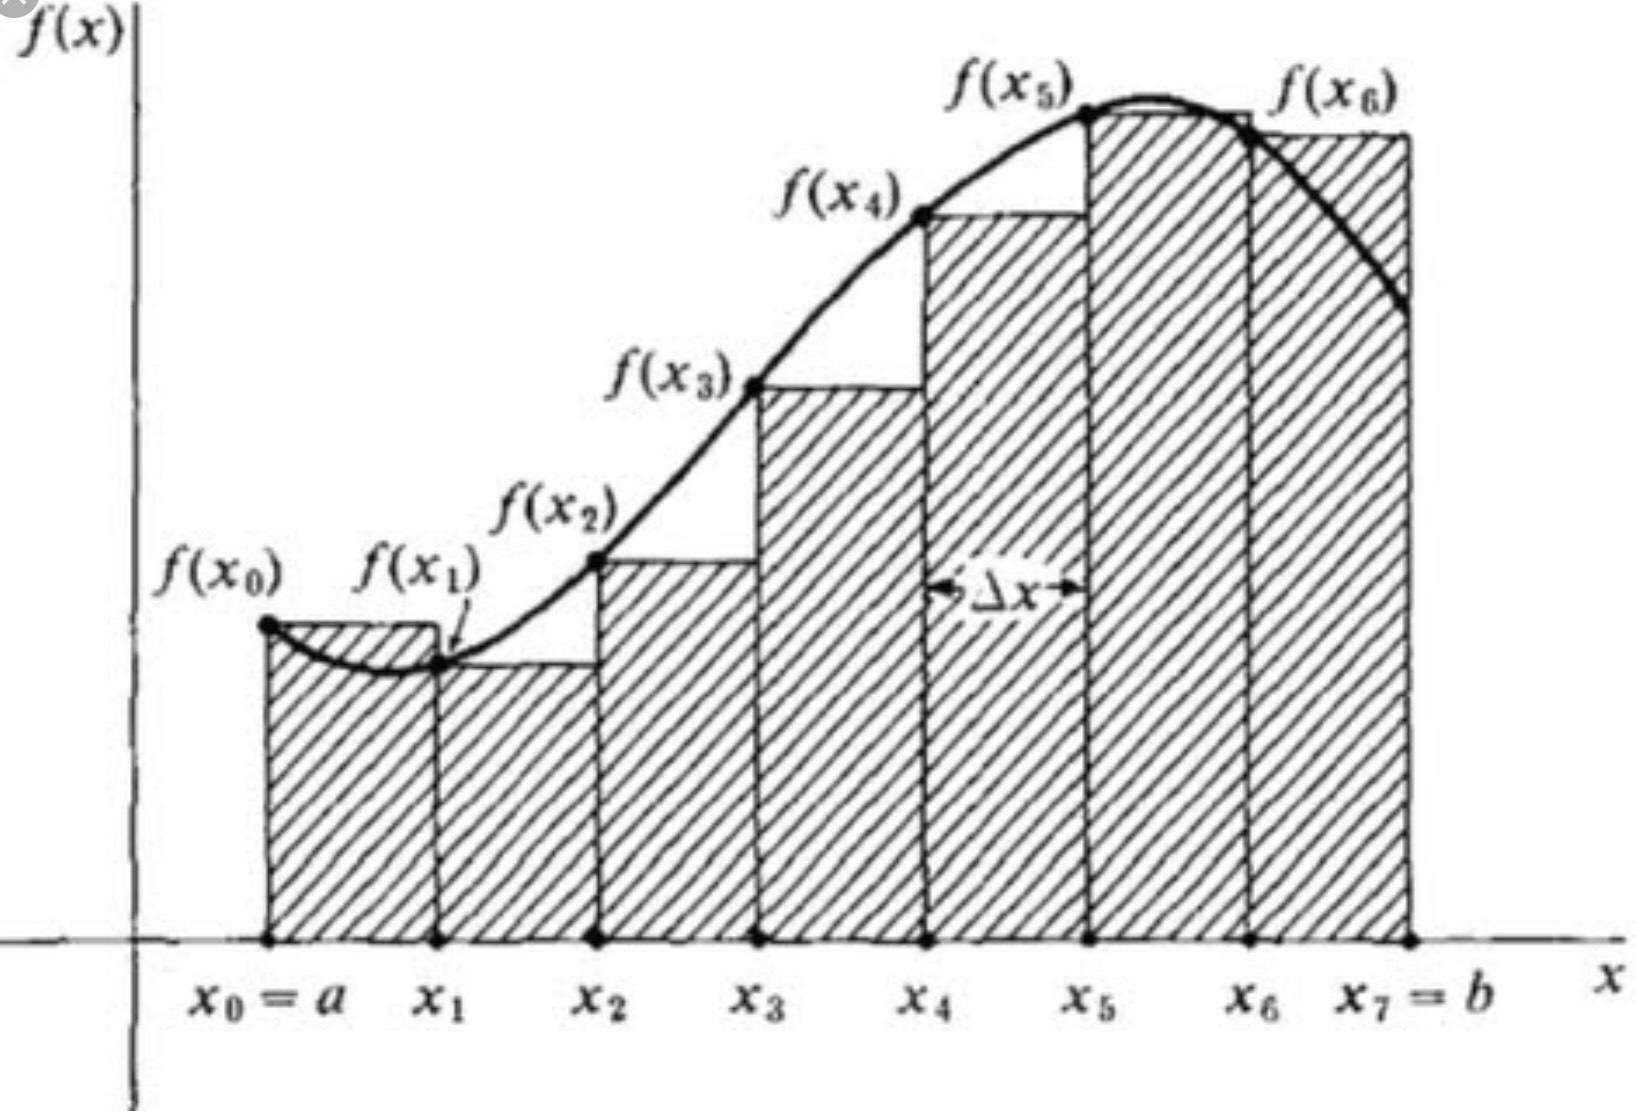
\includegraphics[width=\textwidth]{IMG_0380.jpg}
%		\hspace*{10pt}\hbox{\thinspace{\tiny\itshape vias.org}}
%		\caption{Single integration}
%	\end{subfigure}% 
%	~ 
%	\begin{subfigure}{0.48\textwidth}
%		
%		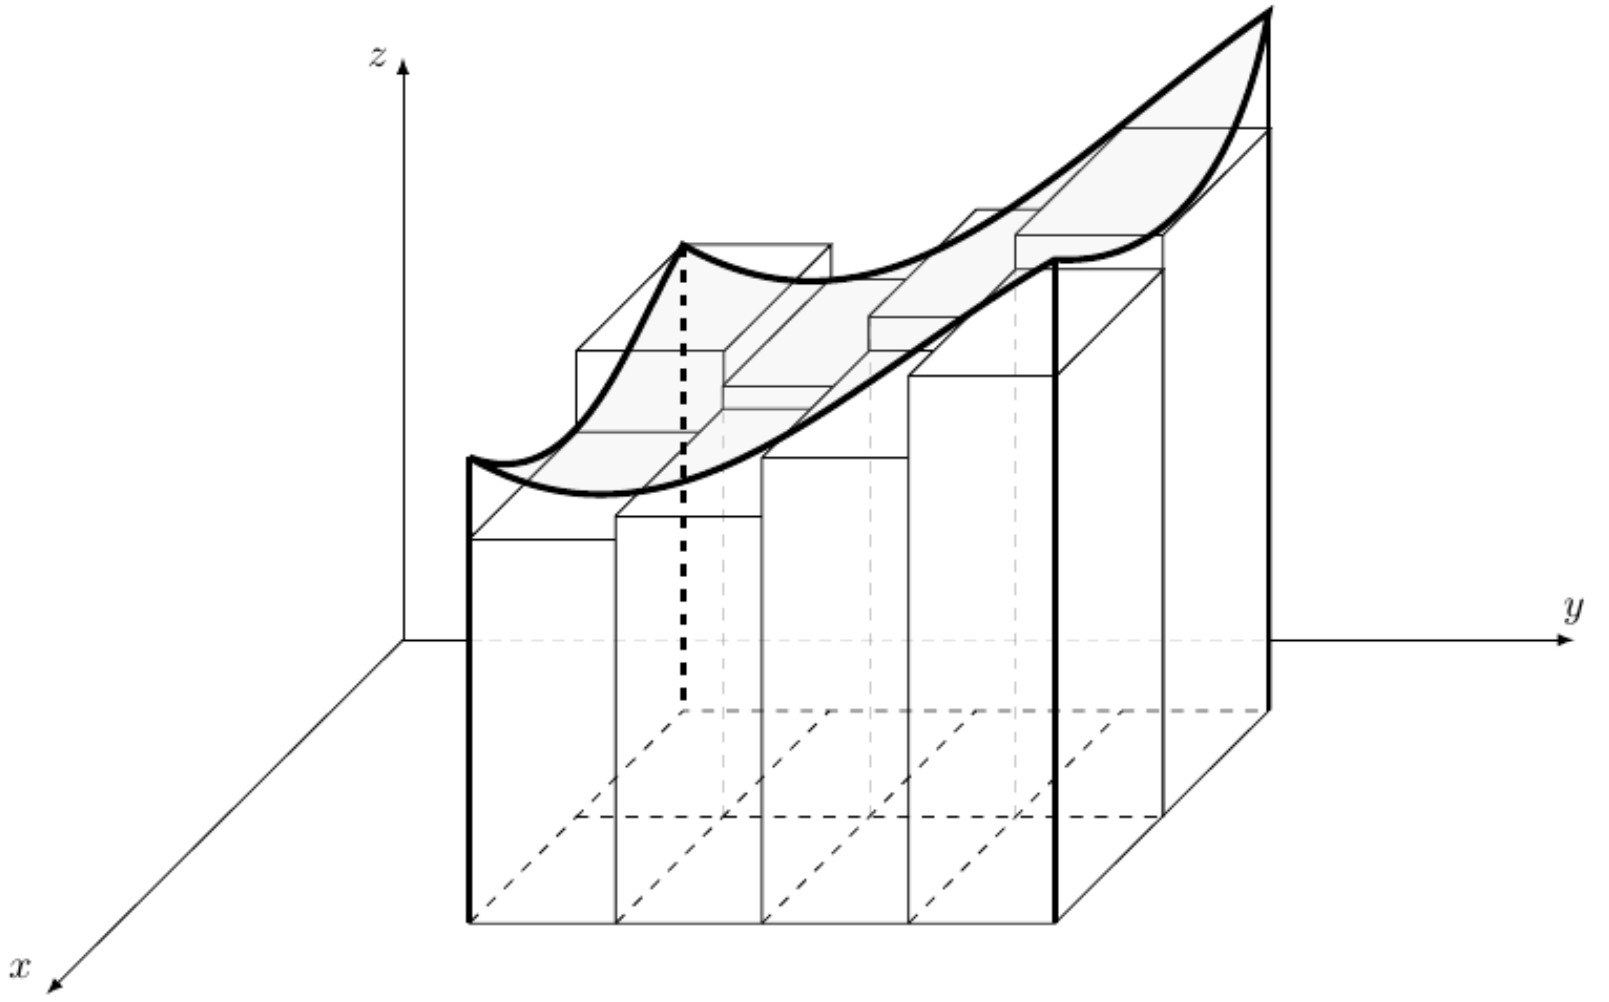
\includegraphics[width=\textwidth]{IMG_0385.jpg}
%		\hspace*{10pt}\hbox{\thinspace{\tiny\itshape tex.stackexchange.com}}
%		\caption{Double integration.}
%		\label{fig:2}
%	\end{subfigure}
%\end{figure}
%
%\end{frame}
%
%
%\begin{frame}
%\frametitle{Triple Integral}
%\begin{figure}
%	\centering
%	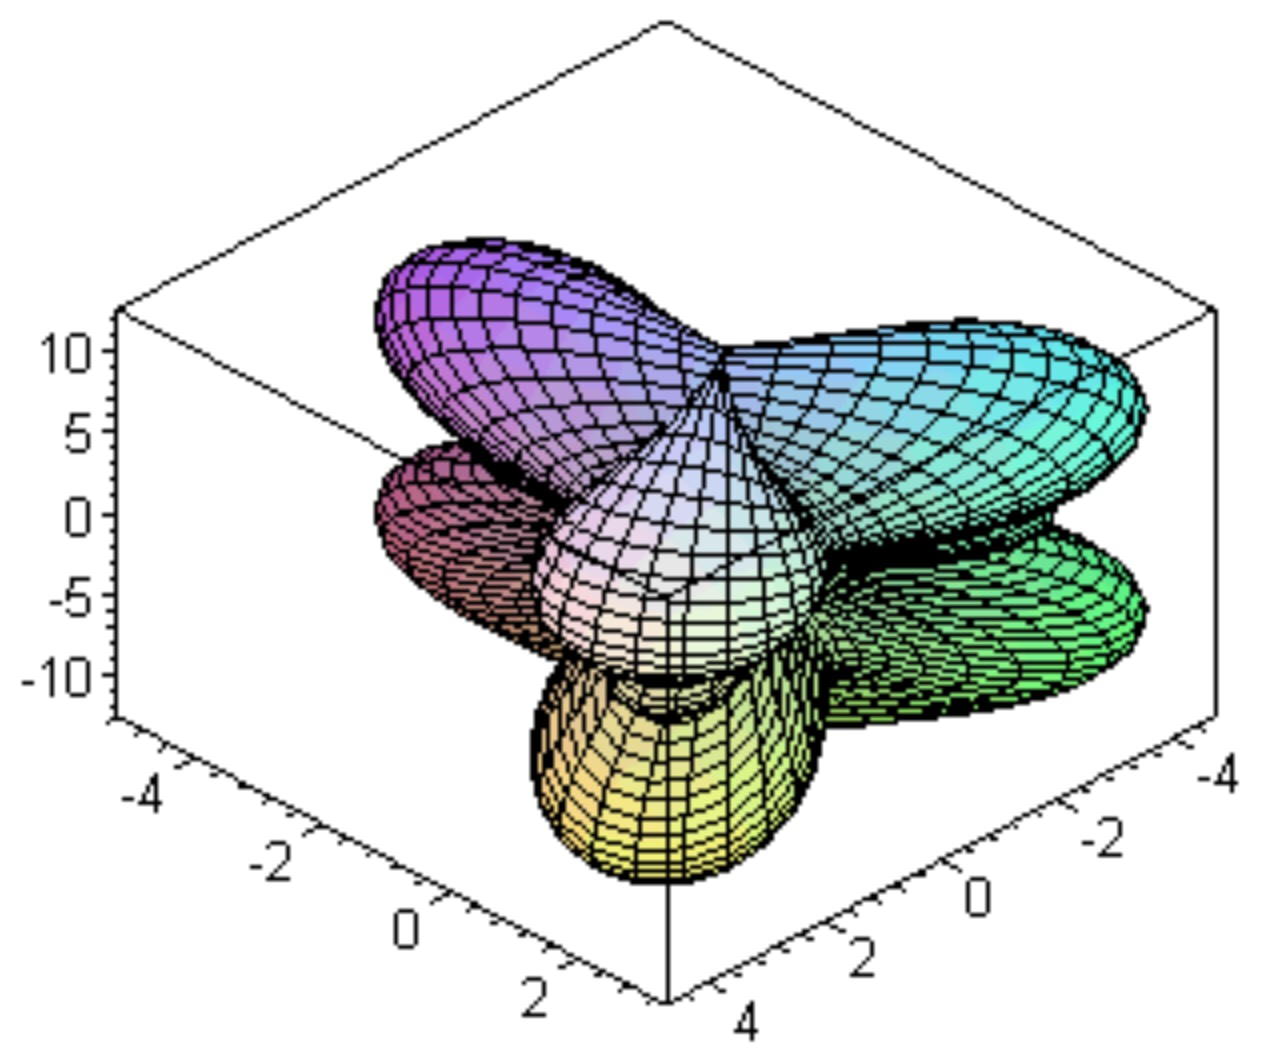
\includegraphics[height=.45\textheight]{IMG_0384.jpg}\\
%	\hspace*{10pt}\hbox{\thinspace{\tiny\itshape maplesoft.com}}
%\end{figure}
%
%$$\iiint\limits_{\mathbb{R}} F(x,y,z) dV = \int_{x=a}^{x=b} \int_{y=y_1(x)}^{y=y_2(x)} \int_{z=z_1(x,y)}^{z=z_2(x,y)} F(x,y,z) dz\,dy\,dx$$
%\textbf{Example:}
%\begin{itemize}
%	\item[(a)] $\int_0^1 \int_0^{1-x} \int_0^{2-x} xyz \,dz\,dy\,dx$
%\end{itemize}
%\end{frame}

\end{document}
